\documentclass[aspectratio=169, 12pt]{beamer}
\usepackage{fontspec}
\setmainfont{Arial}

\usetheme{Madrid}
\usecolortheme{default}

\usepackage{graphicx}
\usepackage{amsmath}
\usepackage{listings}
\usepackage{booktabs}
\usepackage{xcolor}
\usepackage{tabularx}
\usepackage{caption}

% Set code listing style
\lstset{
    basicstyle=\ttfamily\small,
    breaklines=true,
    keywordstyle=\color{blue},
    stringstyle=\color{red},
    commentstyle=\color{green!60!black},
    showstringspaces=false,
    frame=single,
    backgroundcolor=\color{gray!10}
}

\title[ML - Chap 17]{Chương 17: Autoencoder, GAN và Mô hình Khuếch tán}
\author[Giảng viên]{Giảng viên}
\institute[Đại học Đông Á]{Đại học Đông Á}
\date{\today}

\begin{document}

\begin{frame}
    \titlepage
\end{frame}

\begin{frame}{Mục tiêu của Chương}
    \begin{itemize}
        \item Khái quát về Mô hình Không Giám sát và Mô hình Sinh (Generative AI).
        \item Hiểu nguyên lý biểu diễn dữ liệu ẩn qua mạng \textbf{Autoencoder}.
        \item Nắm bắt cơ chế của \textbf{Autoencoder Biến phân (VAE)} để sinh dữ liệu mới.
        \item Tìm hiểu kiến trúc \textbf{Mạng Đối kháng Sinh (GAN)}: Kẻ làm giả và Cảnh sát.
        \item Làm quen với sự tiến hóa của \textbf{Mô hình Khuếch tán (Diffusion Models)} (DDPM, DALL-E, Midjourney).
    \end{itemize}
\end{frame}

\begin{frame}{Mục lục}
    \tableofcontents
\end{frame}

%==================================================================
\section{1. Autoencoder Cơ bản và Biểu diễn Dữ liệu}
%==================================================================

\begin{frame}{1.1 Biểu diễn dữ liệu hiệu quả}
    \begin{itemize}
        \item \textbf{Thí nghiệm trí nhớ cờ vua:} Khi xem một bàn cờ đang chơi, kiện tướng cờ vua nhớ rất nhanh cấu trúc bàn cờ vì họ "nén" thông tin thành các mẫu hình quen thuộc (mở màn phòng thủ Pháp, chuỗi tốt, v.v.).
        \item Con người thường không nhớ chi tiết từng pixel, mà nhớ "ý nghĩa" hoặc "đặc trưng cốt lõi" của nó.
        \item \textbf{Autoencoder} là một mạng nơ-ron học cách \textbf{nén} đầu vào thành một biểu diễn ẩn ngắn gọn, sau đó \textbf{giải nén} nó lại thành dữ liệu ban đầu.
    \end{itemize}
\end{frame}

\begin{frame}{1.2 Kiến trúc Autoencoder Đơn giản}
    \begin{columns}
        \begin{column}{0.4\textwidth}
            \begin{itemize}
                \item Gồm 2 phần:
                \begin{itemize}
                    \item \textbf{Encoder (Mã hóa):} Nhận đầu vào $\mathbf{x}$ và nén thành biểu diễn ẩn $\mathbf{h}$ (latent space).
                    \item \textbf{Decoder (Giải mã):} Dùng $\mathbf{h}$ để phục hồi lại dữ liệu ban đầu $\mathbf{x'}$.
                \end{itemize}
                \item Hàm mất mát là độ sai lệch giữa $\mathbf{x}$ và $\mathbf{x'}$ (MSE Loss).
            \end{itemize}
        \end{column}
        \begin{column}{0.6\textwidth}
            \centering
            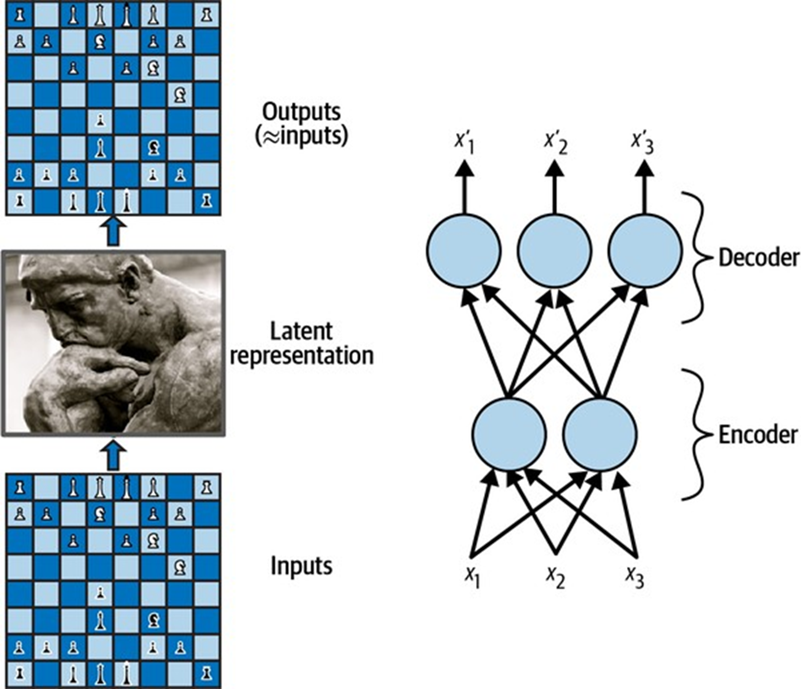
\includegraphics[width=\textwidth,height=0.65\textheight,keepaspectratio]{../machineLearningWeb/Figures/CH17/Hình_17-1.png}
            \vspace{0.2cm}
            \textit{Hình 17-1: Thí nghiệm trí nhớ cờ vua (trái) và Autoencoder (phải)}
        \end{column}
    \end{columns}
\end{frame}

\begin{frame}{1.3 Autoencoder Tuyến tính và PCA}
    \begin{itemize}
        \item \textbf{Autoencoder thiếu hoàn chỉnh (Undercomplete):} Kích thước không gian ẩn (số lượng nơ-ron lớp giữa) nhỏ hơn kích thước đầu vào. Điều này ép mạng phải "học" cách nén.
        \item Nếu Autoencoder chỉ có 1 lớp ẩn và dùng hàm kích hoạt \textbf{tuyến tính} (linear), nó sẽ thực hiện một phép tính tương đương với \textbf{Phân tích Thành phần Chính (PCA)}.
    \end{itemize}
\end{frame}

\begin{frame}{1.4 So sánh PCA và Autoencoder Tuyến tính}
    \begin{columns}
        \begin{column}{0.4\textwidth}
            \begin{itemize}
                \item Bằng cách huấn luyện AE tuyến tính với MSE, mặt phẳng chiếu dữ liệu sẽ giống hệt mặt phẳng được tạo bởi PCA.
                \item AE linh hoạt hơn PCA nhờ khả năng mở rộng thành các mô hình phi tuyến (khi sử dụng hàm kích hoạt ReLU, Sigmoid).
            \end{itemize}
        \end{column}
        \begin{column}{0.6\textwidth}
            \centering
            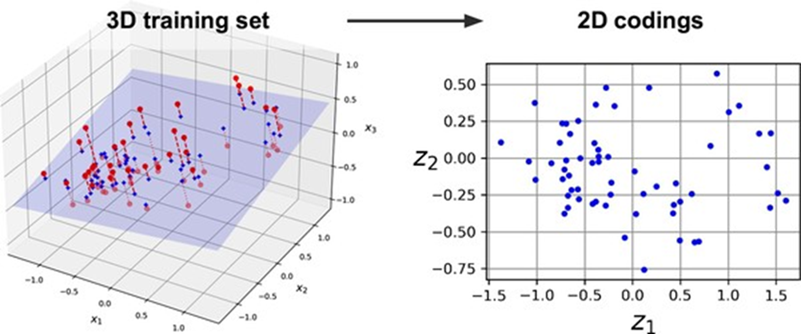
\includegraphics[width=\textwidth,height=0.65\textheight,keepaspectratio]{../machineLearningWeb/Figures/CH17/Hình_17-2.png}
            \vspace{0.2cm}
            \textit{Hình 17-2: Phép chiếu dữ liệu bằng PCA (trái) và AE tuyến tính (phải)}
        \end{column}
    \end{columns}
\end{frame}

\begin{frame}{1.5 Autoencoder Xếp chồng (Stacked Autoencoders)}
    \begin{columns}
        \begin{column}{0.45\textwidth}
            \begin{itemize}
                \item Giống như mạng MLP thông thường, ta có thể xếp chồng nhiều lớp ẩn để Autoencoder học được các đặc trưng phức tạp hơn.
                \item Kiến trúc \textbf{đối xứng}: Encoder nén dần kích thước (vd: 784 $\rightarrow$ 100 $\rightarrow$ 30), Decoder mở rộng lại tương ứng (30 $\rightarrow$ 100 $\rightarrow$ 784).
            \end{itemize}
        \end{column}
        \begin{column}{0.55\textwidth}
            \centering
            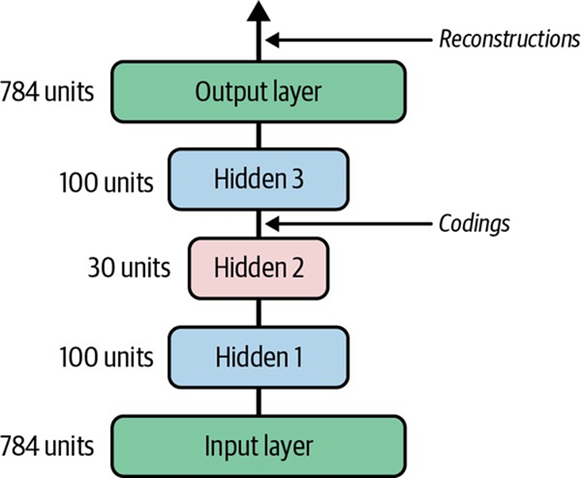
\includegraphics[width=\textwidth,height=0.65\textheight,keepaspectratio]{../machineLearningWeb/Figures/CH17/Hình_17-3.png}
            \vspace{0.2cm}
            \textit{Hình 17-3: Kiến trúc Autoencoder xếp chồng nhiều lớp}
        \end{column}
    \end{columns}
\end{frame}

\begin{frame}[fragile]{1.6 Xây dựng Stacked AE bằng Keras}
    \begin{itemize}
        \item Ví dụ huấn luyện trên bộ dữ liệu Fashion MNIST.
    \end{itemize}
\begin{lstlisting}[language=Python]
stacked_encoder = keras.models.Sequential([
    keras.layers.Flatten(input_shape=[28, 28]),
    keras.layers.Dense(100, activation="selu"),
    keras.layers.Dense(30, activation="selu"),
])
stacked_decoder = keras.models.Sequential([
    keras.layers.Dense(100, activation="selu", input_shape=[30]),
    keras.layers.Dense(28 * 28, activation="sigmoid"),
    keras.layers.Reshape([28, 28])
])
stacked_ae = keras.models.Sequential([stacked_encoder, stacked_decoder])
stacked_ae.compile(loss="binary_crossentropy", optimizer=keras.optimizers.SGD(lr=1.5))
\end{lstlisting}
\end{frame}

\begin{frame}{1.7 Đánh giá Chất lượng Tái tạo (Reconstructions)}
    \begin{columns}
        \begin{column}{0.4\textwidth}
            \begin{itemize}
                \item Để kiểm tra xem AE nén dữ liệu tốt không, ta đưa ảnh vào mạng và xem ảnh giải nén ra.
                \item Dù đã nén từ 784 pixel xuống còn 30 số, AE vẫn giữ được màu sắc và hình dạng cơ bản của chiếc áo/giày.
            \end{itemize}
        \end{column}
        \begin{column}{0.6\textwidth}
            \centering
            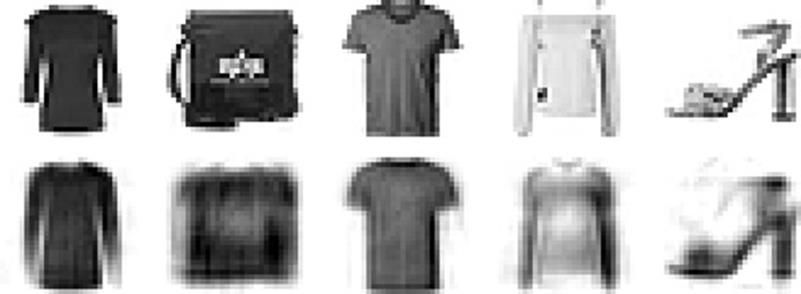
\includegraphics[width=\textwidth,height=0.65\textheight,keepaspectratio]{../machineLearningWeb/Figures/CH17/Hình_17-4.jpg}
            \vspace{0.2cm}
            \textit{Hình 17-4: Hình ảnh gốc (trên) và các bản tái tạo của chúng (dưới)}
        \end{column}
    \end{columns}
\end{frame}

%==================================================================
\section{2. Kỹ thuật nâng cao với Autoencoder}
%==================================================================

\begin{frame}{2.1 Trực quan hóa dữ liệu (Visualization)}
    \begin{itemize}
        \item Không gian ẩn (Latent Space) là tập hợp các tọa độ biểu diễn dữ liệu. Nếu chiều nén là 2 hoặc 3, ta có thể vẽ lên đồ thị trực tiếp.
        \item \textbf{Mẹo thực tế:} Nếu dùng AE giảm về 30 chiều, sau đó áp dụng \textbf{t-SNE} để giảm từ 30 xuống 2 chiều, ta sẽ được biểu đồ phân cụm (Clustering) cực kỳ rõ nét.
    \end{itemize}
\end{frame}

\begin{frame}{2.2 Biểu đồ phân cụm bằng AE + t-SNE}
    \begin{columns}
        \begin{column}{0.4\textwidth}
            \begin{itemize}
                \item Các lớp quần áo giống nhau sẽ nằm cùng một cụm.
                \item Autoencoder đóng vai trò là công cụ trích xuất đặc trưng (Feature Extractor) cực mạnh, ngay cả khi không có nhãn dữ liệu (Unsupervised).
            \end{itemize}
        \end{column}
        \begin{column}{0.6\textwidth}
            \centering
            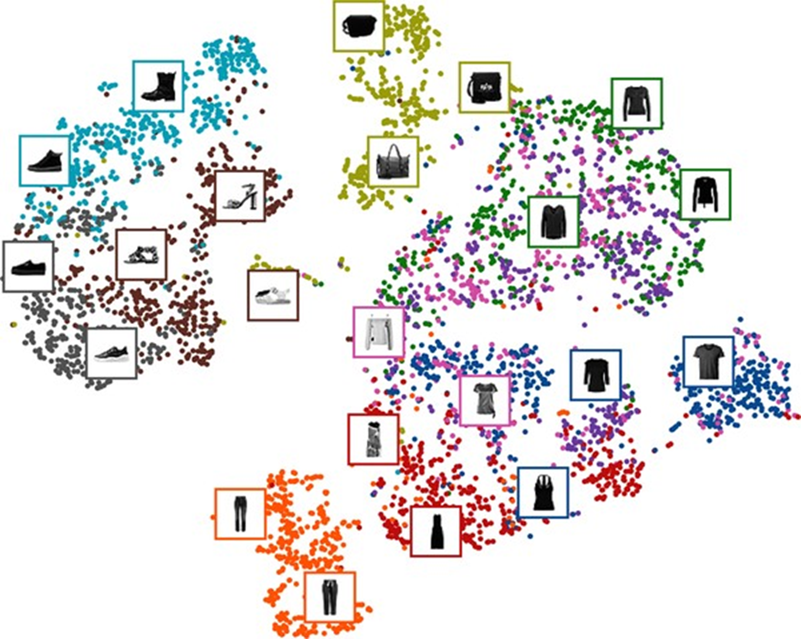
\includegraphics[width=\textwidth,height=0.7\textheight,keepaspectratio]{../machineLearningWeb/Figures/CH17/Hình_17-5.png}
            \vspace{0.2cm}
            \textit{Hình 17-5: Trực quan hóa Fashion MNIST bằng Autoencoder + t-SNE}
        \end{column}
    \end{columns}
\end{frame}

\begin{frame}{2.3 Tiền huấn luyện Không giám sát (Unsupervised Pretraining)}
    \begin{columns}
        \begin{column}{0.4\textwidth}
            \begin{itemize}
                \item Nếu bạn có ít dữ liệu có nhãn nhưng có rất nhiều dữ liệu không gán nhãn, hãy dùng Autoencoder!
                \item Huấn luyện AE trên dữ liệu không nhãn.
                \item Dùng phần \textbf{Encoder} đã huấn luyện để làm các lớp khởi tạo cho bài toán phân loại có giám sát.
            \end{itemize}
        \end{column}
        \begin{column}{0.6\textwidth}
            \centering
            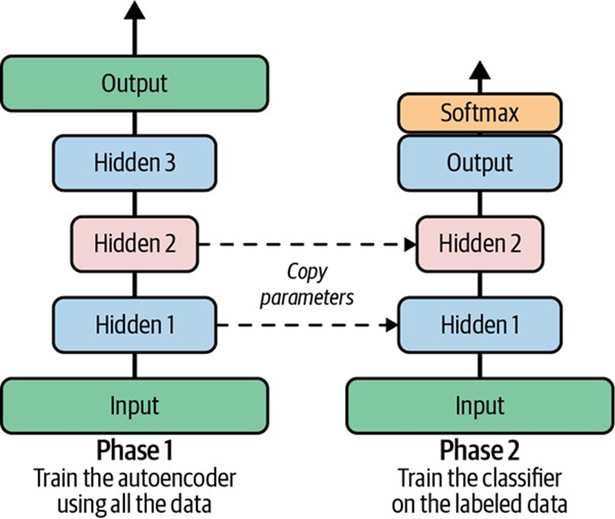
\includegraphics[width=\textwidth,height=0.7\textheight,keepaspectratio]{../machineLearningWeb/Figures/CH17/Hình_17-6.png}
            \vspace{0.2cm}
            \textit{Hình 17-6: Chuyển giao trọng số từ Autoencoder}
        \end{column}
    \end{columns}
\end{frame}

\begin{frame}{2.4 Kỹ thuật Ràng buộc Trọng số (Tying Weights)}
    \begin{itemize}
        \item Autoencoder có cấu trúc đối xứng. Ta có thể \textbf{ép} trọng số của Decoder bằng chính ma trận trọng số chuyển vị của Encoder.
        \item Lợi ích: Giảm một nửa số lượng tham số cần huấn luyện, giúp huấn luyện nhanh hơn và giảm nguy cơ Overfitting.
    \end{itemize}
\end{frame}

\begin{frame}{2.5 Huấn luyện Từng lớp (Greedy Layer-wise Training)}
    \begin{columns}
        \begin{column}{0.4\textwidth}
            \begin{itemize}
                \item Trước kia, khi phần cứng còn yếu, người ta huấn luyện từng AE nông (shallow), sau đó chồng chúng lên nhau để tạo thành Stacked AE.
                \item Ngày nay ta ít dùng, nhưng đây là một kỹ thuật lịch sử vô cùng quan trọng của Deep Learning sơ khai.
            \end{itemize}
        \end{column}
        \begin{column}{0.6\textwidth}
            \centering
            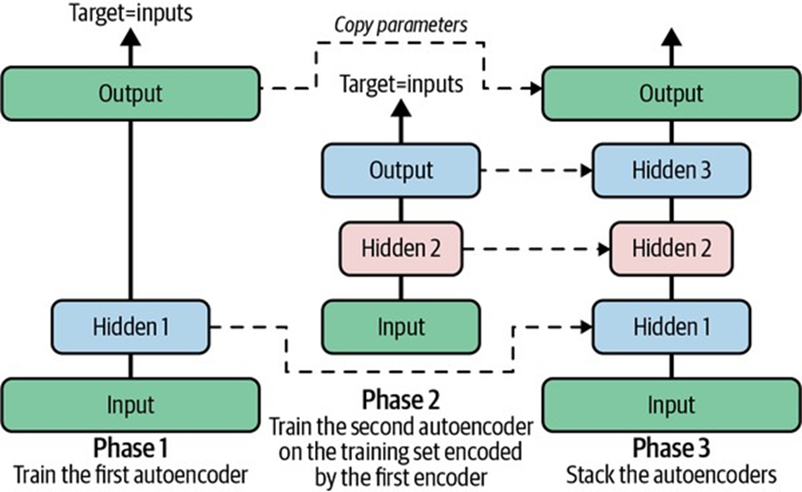
\includegraphics[width=\textwidth,height=0.7\textheight,keepaspectratio]{../machineLearningWeb/Figures/CH17/Hình_17-7.png}
            \vspace{0.2cm}
            \textit{Hình 17-7: Huấn luyện từng Autoencoder riêng lẻ}
        \end{column}
    \end{columns}
\end{frame}

\begin{frame}{2.6 Autoencoder Tích chập (Convolutional AE)}
    \begin{itemize}
        \item Khi làm việc với hình ảnh, các lớp Dense (MLP) phá vỡ cấu trúc không gian của pixel.
        \item Thay vì dùng Dense, ta dùng:
            \begin{itemize}
                \item \textbf{Encoder:} `Conv2D` và `MaxPooling2D` để nén ảnh.
                \item \textbf{Decoder:} `Conv2DTranspose` (hoặc UpSampling2D) để giải nén ảnh.
            \end{itemize}
    \end{itemize}
\end{frame}

\begin{frame}{2.7 Autoencoder Khử nhiễu (Denoising AE)}
    \begin{columns}
        \begin{column}{0.45\textwidth}
            \begin{itemize}
                \item Làm sao ép mạng học được những đặc trưng sâu sắc thay vì chỉ sao chép y nguyên đầu vào?
                \item \textbf{Denoising AE:} Cố tình làm hỏng đầu vào (thêm nhiễu Gaussian, hoặc Dropout vài pixel) nhưng bắt mạng phải tái tạo lại \textbf{ảnh gốc chưa bị nhiễu}.
            \end{itemize}
        \end{column}
        \begin{column}{0.55\textwidth}
            \centering
            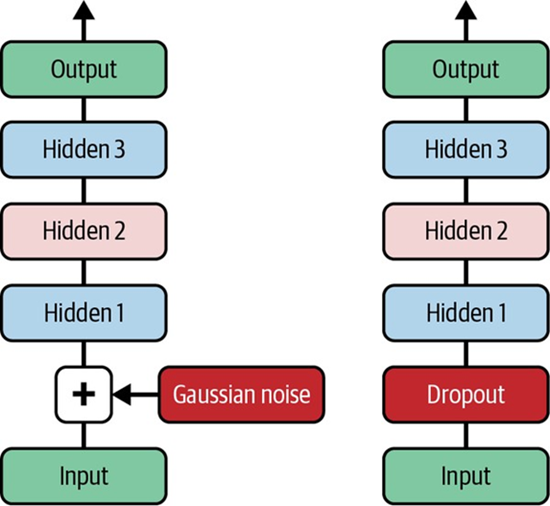
\includegraphics[width=\textwidth,height=0.65\textheight,keepaspectratio]{../machineLearningWeb/Figures/CH17/Hình_17-8.png}
            \vspace{0.2cm}
            \textit{Hình 17-8: Denoising AE với nhiễu Gaussian hoặc Dropout}
        \end{column}
    \end{columns}
\end{frame}

\begin{frame}{2.8 Hiệu quả của Denoising Autoencoder}
    \begin{columns}
        \begin{column}{0.4\textwidth}
            \begin{itemize}
                \item Hình bên cho thấy ảnh đầu vào bị mất 50\% pixel (do Dropout).
                \item Nhưng mạng vẫn phục hồi được hình dáng đôi giày, cái áo. Nó đã thực sự "hiểu" cái áo trông như thế nào.
            \end{itemize}
        \end{column}
        \begin{column}{0.6\textwidth}
            \centering
            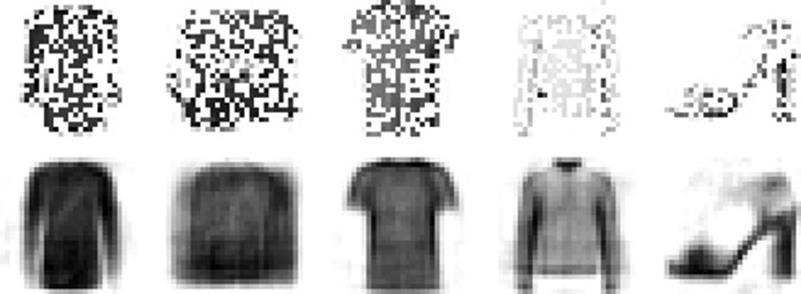
\includegraphics[width=\textwidth,height=0.7\textheight,keepaspectratio]{../machineLearningWeb/Figures/CH17/Hình_17-9.jpg}
            \vspace{0.2cm}
            \textit{Hình 17-9: Hình ảnh bị nhiễu (trên) và bản tái tạo (dưới)}
        \end{column}
    \end{columns}
\end{frame}

\begin{frame}{2.9 Autoencoder Thưa (Sparse AE)}
    \begin{columns}
        \begin{column}{0.5\textwidth}
            \begin{itemize}
                \item Thêm một ràng buộc (penalty) vào hàm mất mát để ép hầu hết các nơ-ron ở lớp Coding (Lớp nén) phải ở trạng thái "tắt" (hoạt động = 0).
                \item Mỗi nơ-ron chỉ được bật lên với một tỷ lệ nhất định (ví dụ 10\%).
                \item Sử dụng \textbf{Kullback-Leibler Divergence (KL Loss)} để ép phân phối hoạt động của nơ-ron về giá trị mục tiêu.
            \end{itemize}
        \end{column}
        \begin{column}{0.5\textwidth}
            \centering
            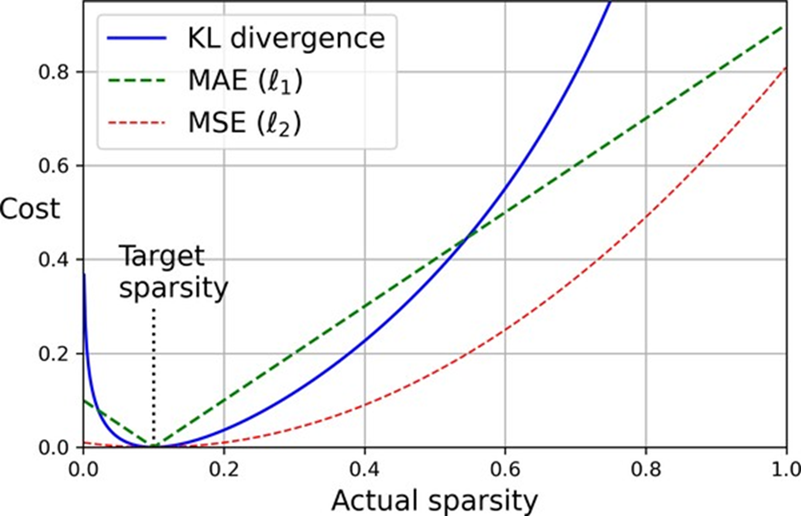
\includegraphics[width=\textwidth,height=0.55\textheight,keepaspectratio]{../machineLearningWeb/Figures/CH17/Hình_17-10.png}
            \vspace{0.2cm}
            \textit{Hình 17-10: Minh họa hình phạt thưa (Sparsity Loss)}
        \end{column}
    \end{columns}
\end{frame}

%==================================================================
\section{3. Autoencoder Biến phân (Variational Autoencoders - VAEs)}
%==================================================================

\begin{frame}{3.1 Giới thiệu về Mô hình Sinh (Generative Models)}
    \begin{itemize}
        \item Autoencoder bình thường chỉ giỏi mã hóa dữ liệu cũ. Nếu ta truyền một Véc-tơ ngẫu nhiên vào Decoder, nó sẽ tạo ra những hình ảnh rất xấu (nhiễu).
        \item \textbf{Mô hình Sinh (Generative Model):} Có khả năng tự \textbf{sáng tạo} ra dữ liệu hoàn toàn mới, trông giống hệt dữ liệu huấn luyện.
        \item \textbf{VAE (Variational Autoencoder)} (2013) là mô hình phổ biến đầu tiên làm được điều này.
    \end{itemize}
\end{frame}

\begin{frame}{3.2 Kiến trúc VAE - Sinh dữ liệu qua Phân phối}
    \begin{columns}
        \begin{column}{0.5\textwidth}
            \begin{itemize}
                \item Thay vì nén ra một giá trị cố định, Encoder của VAE nén ra một \textbf{Phân phối Xác suất} (Giá trị trung bình $\mu$ và Độ lệch chuẩn $\sigma$).
                \item Sau đó, ta \textbf{Lấy mẫu ngẫu nhiên (Sample)} một véc-tơ từ phân phối đó và đưa cho Decoder.
                \item Nghĩa là, cùng một hình ảnh, VAE sẽ giải mã ra các cấu trúc hơi khác nhau đôi chút. Không gian ẩn được làm mượt.
            \end{itemize}
        \end{column}
        \begin{column}{0.5\textwidth}
            \centering
            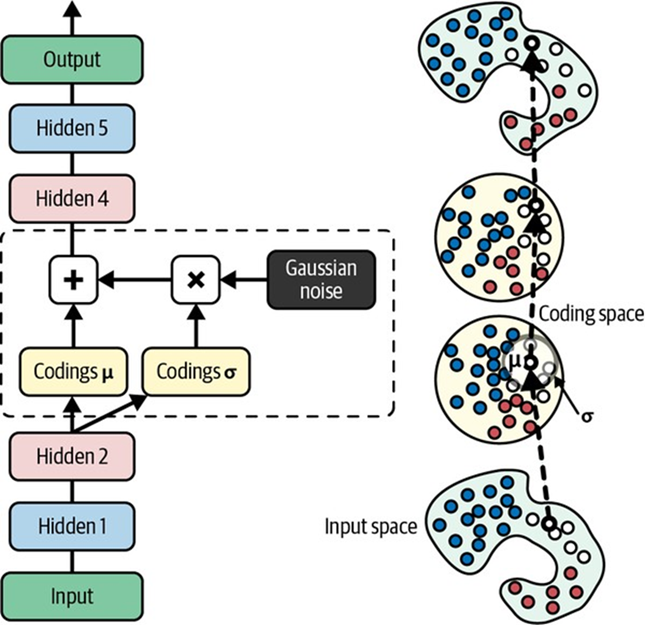
\includegraphics[width=\textwidth,height=0.65\textheight,keepaspectratio]{../machineLearningWeb/Figures/CH17/Hình_17-11.png}
            \vspace{0.2cm}
            \textit{Hình 17-11: Cấu trúc xác suất của VAE}
        \end{column}
    \end{columns}
\end{frame}

\begin{frame}{3.3 Hàm mất mát của VAE và Reparameterization}
    \begin{itemize}
        \item \textbf{Hàm mất mát của VAE gồm 2 phần:}
            \begin{itemize}
                \item Mất mát tái tạo (Reconstruction Loss): Bắt Decoder tái tạo giống ảnh gốc.
                \item Mất mát KL (KL Divergence Loss): Ép phân phối $(\mu, \sigma)$ mà Encoder học được trở nên giống với phân phối Chuẩn (Normal Distribution).
            \end{itemize}
        \item \textbf{Thủ thuật tái tham số hóa (Reparameterization Trick):} Đưa hàm Random ra khỏi đường truyền của Backpropagation để mạng có thể tính đạo hàm bình thường.
    \end{itemize}
\end{frame}

\begin{frame}{3.4 Kết quả Tạo ảnh Mới với VAE}
    \begin{columns}
        \begin{column}{0.4\textwidth}
            \begin{itemize}
                \item Giờ đây, ta có thể bỏ hoàn toàn Encoder đi.
                \item Lấy ngẫu nhiên các véc-tơ tọa độ (tuân theo phân phối chuẩn) và ném vào Decoder.
                \item Decoder sẽ "ảo giác" sinh ra những hình ảnh áo, quần chưa từng tồn tại!
            \end{itemize}
        \end{column}
        \begin{column}{0.6\textwidth}
            \centering
            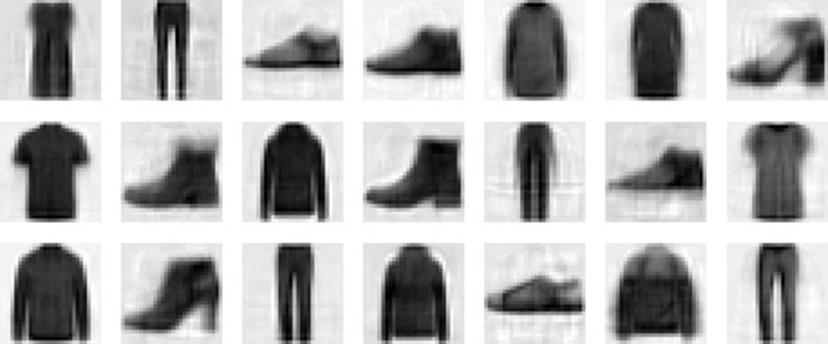
\includegraphics[width=\textwidth,height=0.7\textheight,keepaspectratio]{../machineLearningWeb/Figures/CH17/Hình_17-12.jpg}
            \vspace{0.2cm}
            \textit{Hình 17-12: Ảnh Fashion MNIST hoàn toàn mới được VAE sinh ra}
        \end{column}
    \end{columns}
\end{frame}

\begin{frame}{3.5 Nội suy Ngữ nghĩa (Semantic Interpolation)}
    \begin{columns}
        \begin{column}{0.5\textwidth}
            \begin{itemize}
                \item VAE giữ cho không gian ẩn rất mượt (không có vùng chết).
                \item Nếu ta lấy véc-tơ của "Cái quần" và véc-tơ của "Cái váy", đi từ từ theo đường thẳng nối 2 điểm đó.
                \item Kết quả: Chiếc quần sẽ dần dần biến hóa (morphing) thành chiếc váy một cách tự nhiên.
            \end{itemize}
        \end{column}
        \begin{column}{0.5\textwidth}
            \centering
            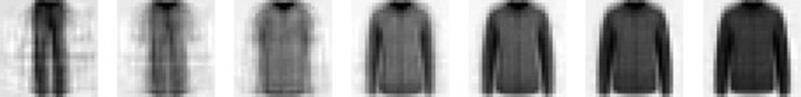
\includegraphics[width=\textwidth,height=0.6\textheight,keepaspectratio]{../machineLearningWeb/Figures/CH17/Hình_17-13.jpg}
            \vspace{0.2cm}
            \textit{Hình 17-13: Sự biến đổi ngữ nghĩa trơn tru trong VAE}
        \end{column}
    \end{columns}
\end{frame}

%==================================================================
\section{4. Mạng Đối kháng Sinh (GANs)}
%==================================================================

\begin{frame}{4.1 Mạng Đối kháng Sinh (Generative Adversarial Networks)}
    \begin{itemize}
        \item Đề xuất bởi Ian Goodfellow (2014), GAN tạo ra cơn địa chấn trong ngành Trí tuệ Nhân tạo.
        \item Khác biệt: GAN không có hàm mất mát đo sai lệch thông thường (MSE). Nó là một \textbf{Trò chơi (Game Theory)} giữa 2 mạng Nơ-ron đấu đá nhau.
    \end{itemize}
\end{frame}

\begin{frame}{4.2 Kiến trúc Kẻ làm giả và Cảnh sát}
    \begin{columns}
        \begin{column}{0.5\textwidth}
            \begin{itemize}
                \item \textbf{Mạng Tạo (Generator):} Kẻ làm giả tiền. Nhận nhiễu ngẫu nhiên và cố gắng sinh ra ảnh giả sao cho chân thực nhất.
                \item \textbf{Mạng Phân biệt (Discriminator):} Cảnh sát. Nhận cả ảnh thật và ảnh giả, cố gắng phân biệt được đâu là thật, đâu là giả.
                \item Cả hai sẽ liên tục tiến bộ, đến khi Generator làm giả tinh vi tới mức Discriminator chỉ còn cách đoán mò (50\%).
            \end{itemize}
        \end{column}
        \begin{column}{0.5\textwidth}
            \centering
            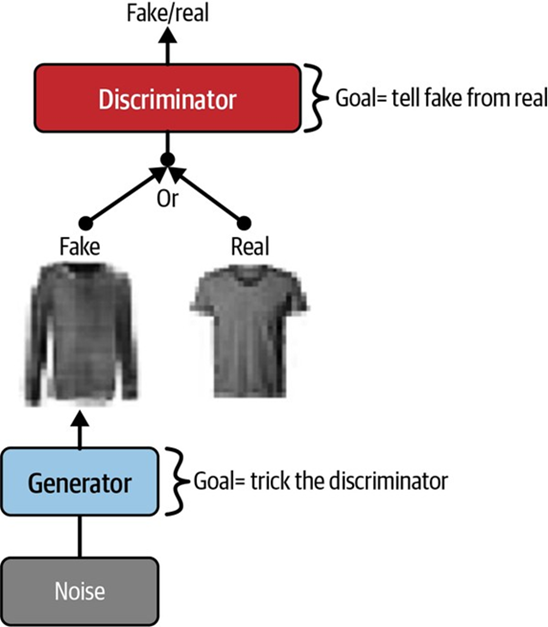
\includegraphics[width=\textwidth,height=0.7\textheight,keepaspectratio]{../machineLearningWeb/Figures/CH17/Hình_17-14.png}
            \vspace{0.2cm}
            \textit{Hình 17-14: Kiến trúc Mạng đối kháng sinh (GAN)}
        \end{column}
    \end{columns}
\end{frame}

\begin{frame}{4.3 Vòng lặp Huấn luyện GAN}
    \begin{itemize}
        \item \textbf{Pha 1 (Huấn luyện Cảnh sát):} Đóng băng Generator. Lấy ảnh thật (gán nhãn 1) và ảnh giả (gán nhãn 0). Huấn luyện Discriminator để dự đoán chuẩn xác.
        \item \textbf{Pha 2 (Huấn luyện Kẻ làm giả):} Đóng băng Discriminator. Bắt Generator sinh ảnh, đưa qua Discriminator và \textbf{gán nhãn mục tiêu là 1 (thật)}. Việc này ép Generator học cách thay đổi tham số để lừa Cảnh sát.
    \end{itemize}
\end{frame}

\begin{frame}{4.4 Hạn chế và Khó khăn của GAN (Vanilla GAN)}
    \begin{columns}
        \begin{column}{0.45\textwidth}
            \begin{itemize}
                \item \textbf{Sụp đổ chế độ (Mode Collapse):} Generator phát hiện ra Cảnh sát thích 1 loại ảnh nhất định (vd: Giày), thế là nó chỉ sinh ra Giày, bỏ qua Quần áo.
                \item \textbf{Gradient mờ nhạt:} Nếu Discriminator quá xuất sắc, nó đập chết Generator ngay từ đầu, Generator không học được gì thêm.
                \item Hình bên: GAN cơ bản (Vanilla) sinh ảnh khá mờ và rung.
            \end{itemize}
        \end{column}
        \begin{column}{0.55\textwidth}
            \centering
            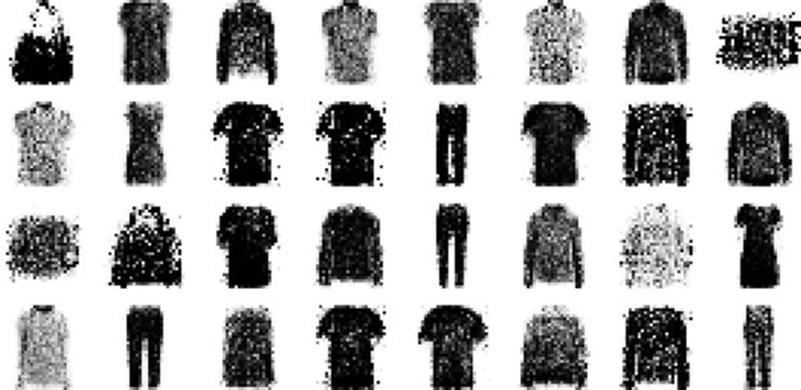
\includegraphics[width=\textwidth,height=0.7\textheight,keepaspectratio]{../machineLearningWeb/Figures/CH17/Hình_17-15.jpg}
            \vspace{0.2cm}
            \textit{Hình 17-15: Ảnh tạo bởi GAN sơ khai thường kém ổn định}
        \end{column}
    \end{columns}
\end{frame}

\begin{frame}{4.5 GAN Tích chập Sâu (DCGANs - 2015)}
    \begin{itemize}
        \item Để sinh ảnh sắc nét, ta kết hợp mạng CNN vào GAN.
        \item Tuy nhiên GAN rất dễ "sập" khi thêm Conv Layer.
        \item \textbf{Kiến trúc DCGAN tiêu chuẩn:}
            \begin{itemize}
                \item Bỏ tất cả lớp Pooling, thay bằng Strided Convolutions.
                \item Thêm \textbf{Batch Normalization} cho cả Generator và Discriminator.
                \item Generator dùng \textbf{ReLU}, nhưng Discriminator bắt buộc dùng \textbf{LeakyReLU}.
                \item Loại bỏ các lớp Dense ẩn.
            \end{itemize}
    \end{itemize}
\end{frame}

\begin{frame}{4.6 Kết quả ấn tượng của DCGAN}
    \begin{columns}
        \begin{column}{0.4\textwidth}
            \begin{itemize}
                \item Với kiến trúc trên, GAN ổn định hơn hẳn.
                \item Hình bên là kết quả sau 50 epochs huấn luyện trên Fashion MNIST.
                \item Hình ảnh sắc nét và đa dạng, ít bị Mode Collapse hơn.
            \end{itemize}
        \end{column}
        \begin{column}{0.6\textwidth}
            \centering
            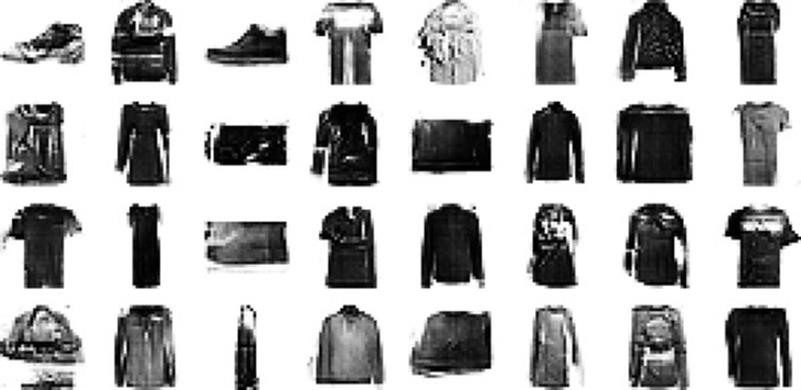
\includegraphics[width=\textwidth,height=0.7\textheight,keepaspectratio]{../machineLearningWeb/Figures/CH17/Hình_17-16.jpg}
            \vspace{0.2cm}
            \textit{Hình 17-16: DCGAN mang lại chất lượng ảnh sắc nét hơn}
        \end{column}
    \end{columns}
\end{frame}

\begin{frame}{4.7 Toán học Không gian Ẩn của GAN}
    \begin{columns}
        \begin{column}{0.5\textwidth}
            \begin{itemize}
                \item Không gian véc-tơ mà GAN học được rất có cấu trúc.
                \item Ta có thể làm \textbf{Toán học} trên các bức ảnh!
                \item Ví dụ: Véc-tơ(Người đàn ông đeo kính) - Véc-tơ(Đàn ông) + Véc-tơ(Phụ nữ) = Véc-tơ(Phụ nữ đeo kính).
                \item Máy tính đã tự hiểu khái niệm "Kính" là gì!
            \end{itemize}
        \end{column}
        \begin{column}{0.5\textwidth}
            \centering
            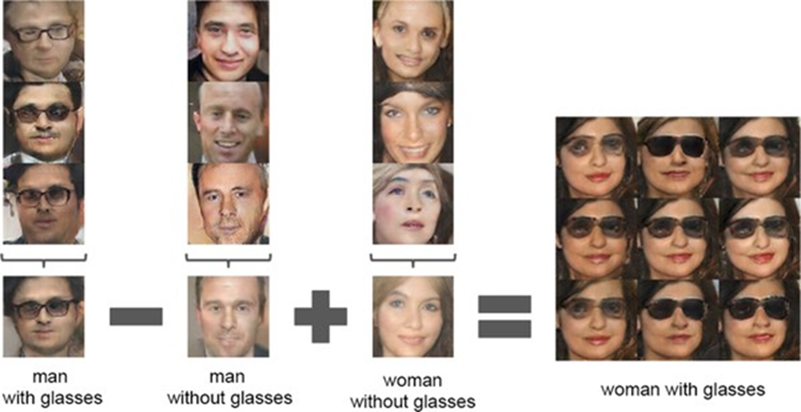
\includegraphics[width=\textwidth,height=0.6\textheight,keepaspectratio]{../machineLearningWeb/Figures/CH17/Hình_17-17.png}
            \vspace{0.2cm}
            \textit{Hình 17-17: Phép toán Véc-tơ trên Khái niệm Hình ảnh}
        \end{column}
    \end{columns}
\end{frame}

\begin{frame}{4.8 Sự phát triển tăng dần của GANs (ProGANs)}
    \begin{columns}
        \begin{column}{0.45\textwidth}
            \begin{itemize}
                \item \textbf{Vấn đề:} Sinh ảnh khuôn mặt $1024 \times 1024$ từ con số 0 là quá sức với Generator (quá nhiều Pixel, Discriminator sẽ nhận ra ngay).
                \item \textbf{Giải pháp:} Bắt đầu bằng ảnh $4 \times 4$. Khi mạng hội tụ, ta từ từ thêm các lớp Convolution để tăng lên $8 \times 8$, rồi $16 \times 16$, cho tới độ phân giải 4K.
            \end{itemize}
        \end{column}
        \begin{column}{0.55\textwidth}
            \centering
            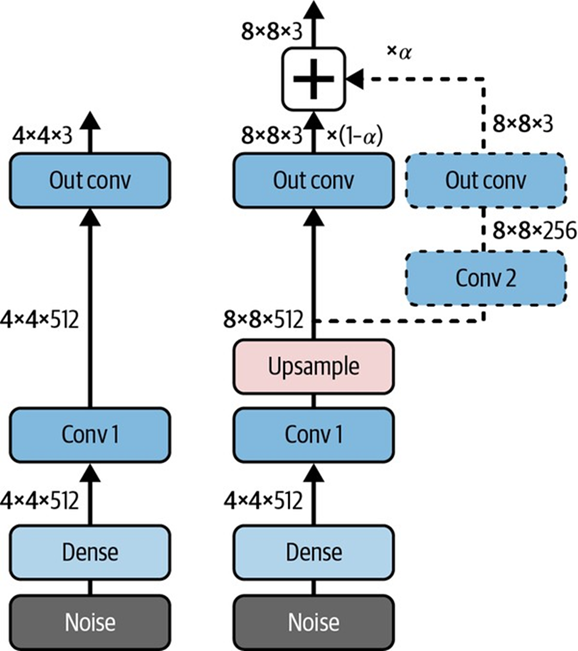
\includegraphics[width=\textwidth,height=0.65\textheight,keepaspectratio]{../machineLearningWeb/Figures/CH17/Hình_17-18.png}
            \vspace{0.2cm}
            \textit{Hình 17-18: Kỹ thuật nhét dần các lớp độ phân giải cao vào GAN}
        \end{column}
    \end{columns}
\end{frame}

\begin{frame}{4.9 StyleGAN (2018) - Định nghĩa lại Chất lượng sinh ảnh}
    \begin{columns}
        \begin{column}{0.4\textwidth}
            \begin{itemize}
                \item Kế thừa ProGAN, NVIDIA phát triển StyleGAN.
                \item StyleGAN có thể kiểm soát được đặc điểm khuôn mặt:
                \begin{itemize}
                    \item Cấp vĩ mô: Giới tính, tư thế.
                    \item Cấp vi mô: Màu tóc, tàn nhang.
                \end{itemize}
                \item Đây là công nghệ đằng sau trang web nổi tiếng \textit{"This Person Does Not Exist"}.
            \end{itemize}
        \end{column}
        \begin{column}{0.6\textwidth}
            \centering
            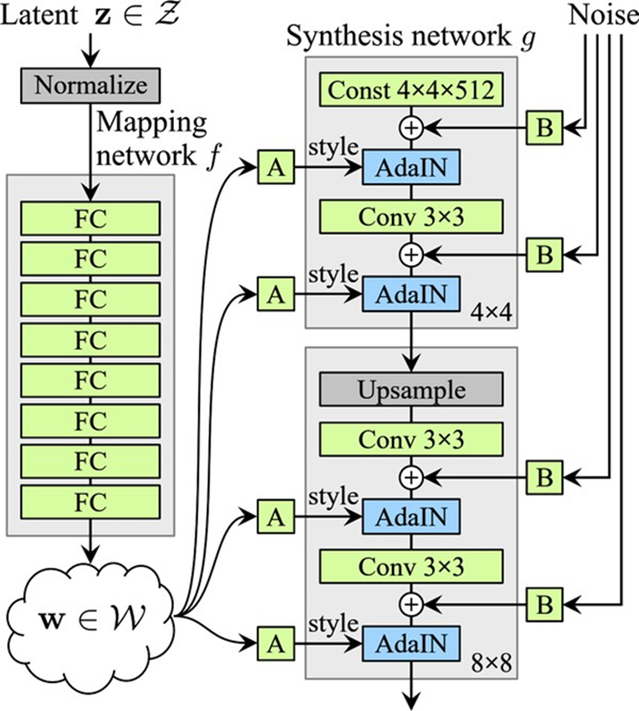
\includegraphics[width=\textwidth,height=0.7\textheight,keepaspectratio]{../machineLearningWeb/Figures/CH17/Hình_17-19.png}
            \vspace{0.2cm}
            \textit{Hình 17-19: Kiến trúc mạng tạo của StyleGAN}
        \end{column}
    \end{columns}
\end{frame}

%==================================================================
\section{5. Mô hình Khuếch tán (Diffusion Models)}
%==================================================================

\begin{frame}{5.1 Kỷ nguyên của Mô hình Khuếch tán (Diffusion Models)}
    \begin{itemize}
        \item GAN rất mạnh nhưng rất "đỏng đảnh" (khó huấn luyện, Mode Collapse, tỷ lệ thất bại cao).
        \item Khoảng năm 2021-2022, thế giới chuyển dịch sang \textbf{Diffusion Models}.
        \item Đây là công nghệ lõi vận hành các AI vẽ tranh đình đám nhất hiện nay: \textbf{Midjourney, Stable Diffusion, DALL-E 3}.
    \end{itemize}
\end{frame}

\begin{frame}{5.2 Nguyên lý: Phá hủy và Phục hồi}
    \begin{columns}
        \begin{column}{0.45\textwidth}
            \begin{itemize}
                \item Lấy cảm hứng từ Nhiệt động lực học (sự khuếch tán phân tử khí).
                \item \textbf{Quá trình tiến (Forward/Diffusion):} Lấy 1 bức ảnh thật, thêm từng chút nhiễu (Gaussian Noise) cho đến khi bức ảnh trở thành một mớ nhiễu trắng hỗn độn.
                \item \textbf{Quá trình ngược (Reverse):} Dạy mạng nơ-ron học cách \textbf{khử nhiễu} từng bước một để lùi về ảnh gốc.
            \end{itemize}
        \end{column}
        \begin{column}{0.55\textwidth}
            \centering
            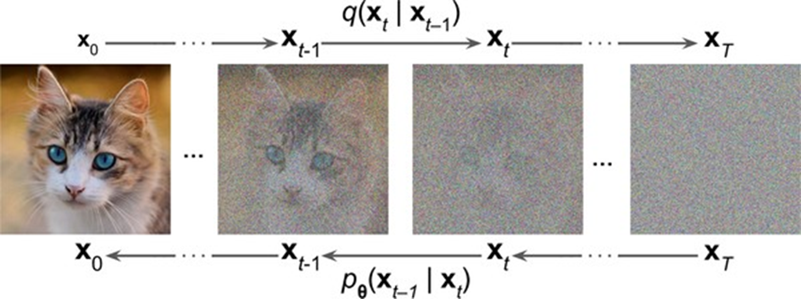
\includegraphics[width=\textwidth,height=0.65\textheight,keepaspectratio]{../machineLearningWeb/Figures/CH17/Hình_17-20.png}
            \vspace{0.2cm}
            \textit{Hình 17-20: Quá trình Phá hủy (q) và Khử nhiễu (p)}
        \end{column}
    \end{columns}
\end{frame}

\begin{frame}{5.3 Lịch trình Phương sai (Variance Schedule)}
    \begin{columns}
        \begin{column}{0.5\textwidth}
            \begin{itemize}
                \item Ta không thêm nhiễu ngẫu nhiên, mà thêm theo lịch trình (ví dụ: $T = 1000$ bước).
                \item Ở bước $t$, tín hiệu gốc giảm đi, lượng nhiễu tăng lên.
                \item Toán học của Chuỗi Markov giúp ta có thể "nhảy" trực tiếp đến bước nhiễu $t$ bất kỳ mà không cần lặp qua từng bước trước đó (công thức $q(x_t|x_0)$).
            \end{itemize}
        \end{column}
        \begin{column}{0.5\textwidth}
            \centering
            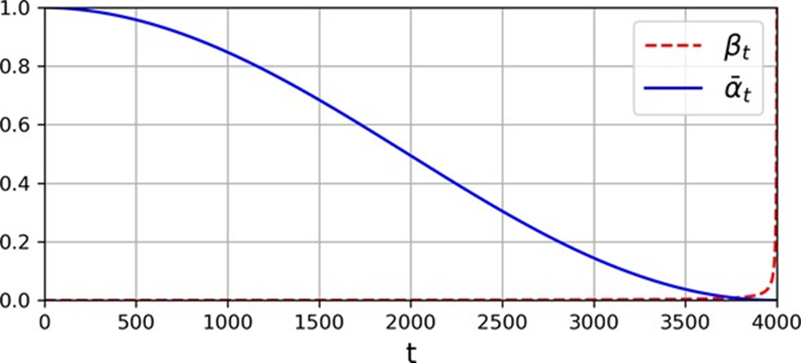
\includegraphics[width=\textwidth,height=0.6\textheight,keepaspectratio]{../machineLearningWeb/Figures/CH17/Hình_17-21.png}
            \vspace{0.2cm}
            \textit{Hình 17-21: Lịch phương sai nhiễu $\beta_t$ và tín hiệu $\bar{\alpha}_t$}
        \end{column}
    \end{columns}
\end{frame}

\begin{frame}{5.4 Denoising Diffusion Probabilistic Models (DDPM)}
    \begin{columns}
        \begin{column}{0.4\textwidth}
            \begin{itemize}
                \item Mạng U-Net được dùng để dự đoán \textbf{Lượng nhiễu} đã được thêm vào ở bước $t$.
                \item Quá trình sinh ảnh: Bắt đầu từ 1 khung ảnh chứa toàn nhiễu TV (như tivi mất sóng). Cho qua U-Net 1000 lần, mỗi lần trừ đi một chút nhiễu.
                \item Kết quả: Bức ảnh thật tuyệt đẹp dần hiện ra!
            \end{itemize}
        \end{column}
        \begin{column}{0.6\textwidth}
            \centering
            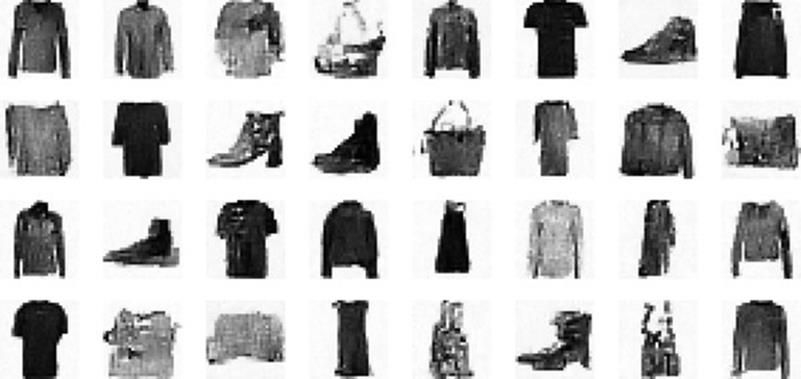
\includegraphics[width=\textwidth,height=0.7\textheight,keepaspectratio]{../machineLearningWeb/Figures/CH17/Hình_17-22.jpg}
            \vspace{0.2cm}
            \textit{Hình 17-22: Hình ảnh sinh vật lạ được tạo bởi DDPM}
        \end{column}
    \end{columns}
\end{frame}

\begin{frame}{Tổng Kết Chương 17}
    \begin{itemize}
        \item \textbf{Autoencoder:} Mô hình học không giám sát mạnh mẽ, nén dữ liệu qua cổ chai. Ứng dụng: Giảm chiều, phân cụm, tiền xử lý.
        \item \textbf{VAE:} Bước đệm sang Mô hình Sinh, nén dữ liệu thành hàm xác suất để sinh ra không gian ảo giác mượt mà.
        \item \textbf{GANs:} Chơi trò chơi cảnh sát - trộm, sinh ra ảnh sắc nét nhất nhưng khó huấn luyện và bảo trì.
        \item \textbf{Diffusion Models:} Phá hủy dữ liệu bằng nhiễu và học cách phục hồi. Tốc độ tạo ảnh chậm hơn GAN nhưng chất lượng và độ đa dạng vượt trội, là tiêu chuẩn công nghiệp hiện nay.
    \end{itemize}
\end{frame}

\begin{frame}
    \centering
    \Huge \textbf{HỎI \& ĐÁP}
\end{frame}

\end{document}
